\subsection{Neural Radiance Fields~--~NeRFs}\label{NeRF}

Neural Radiance Fields (NeRFs), as introduced by \citeauthor{mildenhallNERF}, represent a significant advancement in 3D scene representation, particularly when compared to previous methods which often struggle with complex geometries and varying lighting conditions. Emerging in response to these challenges, NeRFs employ a novel volumetric representation, capturing the spatial and angular distribution of light more accurately \citep{mildenhallNERF}.

\begin{figure}[ht]
    \centering
      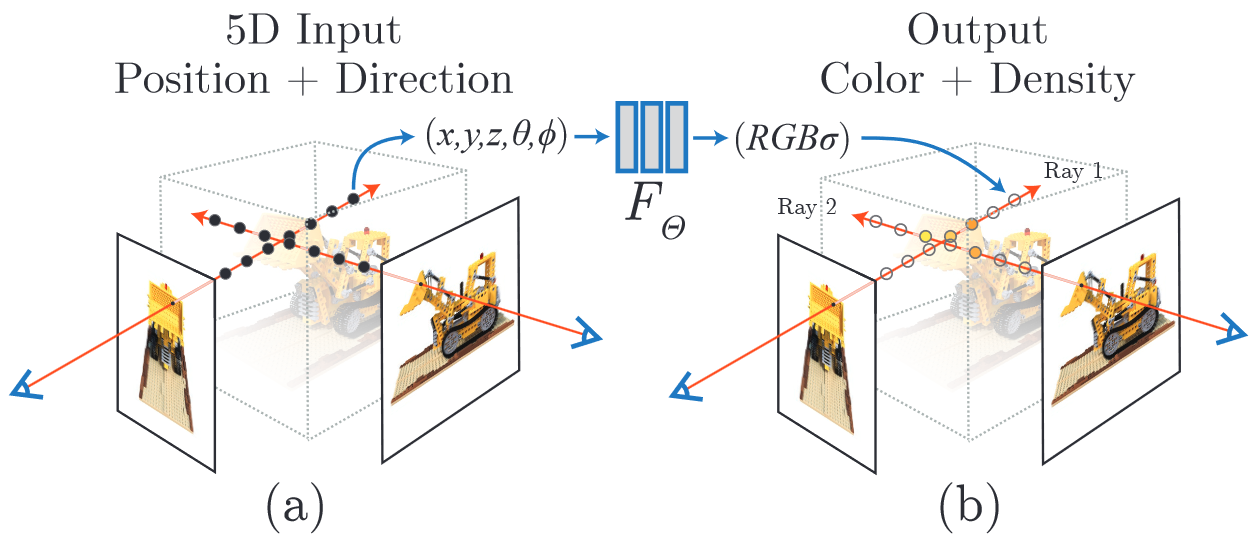
\includegraphics[width=1\columnwidth]{figures/NeRF_Fig_2_Mildenhall.png}
      \caption{Sumamrized workflow of a NeRF as shown in~\citep{mildenhallNERF}: 5D input (Position + Direction) is processed by the MLP \(F_\theta\) to output color and density. Volume rendering integrates predictions along rays to generate an image from the specified viewpoint. The rendering loss, comparing the rendered and actual images, guides the network's training and refinement process.}\label{fig:figureNeRF}
\end{figure}

NeRFs start the generation process by initializing a 3D scene with random values. This serves as a starting point for refining the scene through training a Multilayer Perceptron (MLP) \(F\), parameterized by \(\theta\). The MLP consists of Fully Connected Layers (FCs) with ReLU activations, specifically designed to encode the volumetric details of that particular scene, effectively creating a dedicated neural network for each scene \citep{mildenhallNERF}. The neural network accepts two types of input: a position in a given coordinate system, expressed as a 3D vector \(x, y, z\), and a viewing direction represented by two angles \( \theta, \phi \). Imagine a scenario where a flashlight is held in the middle of a dark room. The angle \( \theta \) would represent how much the flashlight is tilted up or down. Similarly, the angle \( \phi \) would represent how much the flashlight is rotated about the vertical axis while pointed outward. The network's output consists of the color \(c\) and density \( \sigma \) at that particular location \citep{mildenhallNERF}. 

Central to NeRF's operation is the process of volume rendering, which involves casting rays through the scene and gathering color and density information at multiple points.\[ 
C(r) = \int_{t_n}^{t_f} T(t)\sigma(r(t))c(r(t), d)dt \quad \text{where} \quad T(t) = \exp\left(-\int_{t_n}^t \sigma(r(s))ds\right) 
\] This formula, as outlined by \citeauthor{mildenhallNERF}, enables the rendering of a 3D scene by casting rays and aggregating their properties from a near boundary (\(t_n\)) to a far boundary (\(t_f\)). The equation essentially builds up an image by integrating the effects of light interaction with the scene's material over the length of each ray. The volume density \(\sigma\) at a point in the scene indicates the amount of light-blocking material at that specific location. A higher density suggests a greater likelihood of a light ray being obstructed, signifying more material at that point. The accumulated transmittance \( T(t) \) reflects the cumulative effect of density along a ray's path. It quantifies the extent to which light from the start of the ray can travel through the scene to a given point without being absorbed or scattered by the material. Its value decreases along the ray's path as it encounters areas of higher density. The point at which this density curve rises significantly usually corresponds to an object in the scene, and the color \( c(r(t), d) \) at this point is what is rendered for that particular pixel. As seen in Figure~\ref{fig:figureNeRF}, these density and color curves can be visualized to illustrate how density and color vary along the ray's path \citep{mildenhallNERF}. Repeating this ray casting process for every pixel of an image effectively creates \(C(r)\), a 2D ``screenshot'' of the current 3D scene, given the viewing direction \( d \) of where each ray is shot. 

Classical deep learning methods often require a comprehensive dataset of 3D models comprising different scenes and their representations. NeRFs overcome this limitation and rely only on a set of 2D images of the target object from multiple angles that serve as ground truth. After volume rendering, NeRFs compare the newly generated image of the scene with the corresponding real image from the original 2D set. The difference between these images is calculated using the total squared error, which determines the difference between the original and the rendered image \citep{mildenhallNERF}. This loss is then backpropagated to the MLP, which adjusts its parameters in response to this calculated loss aiming to reduce the discrepancy between both images. This iterative adjustment process is applied to all viewing angles of the original data set until the MLP reaches convergence, where the rendered images closely match the real images.

To address multi-view consistency, NeRF predicts color as a function of both location and viewing direction, while density depends solely on location. This separation acknowledges that density, unlike color, remains consistent regardless of viewing angle \citep{hu2023consistentnerf}. 

Although naive NeRF models may not provide photorealistic results due to the lack of detail, several optimizations have been introduced to improve their performance. One notable improvement is the use of positional encoding techniques that deterministically map 3D coordinates and view directions to a higher dimensional space. This is achieved by using high-frequency features before inputting them to the multilayer perceptron (MLP), which helps optimize the neural radiation fields to better represent high-frequency scene content \citep{mildenhallNERF}. Hierarchical volume sampling offers another optimization. This strategy involves two neural network systems, one coarse and one refined, which are jointly optimized during training. Initially, the coarse network sparsely samples the rays in the 3D scene, and based on this initial sampling, a refined network is guided to perform a more detailed sampling. This hierarchical approach is beneficial because dense sampling is very computationally expensive. A two-tier system therefore helps manage computational resources while allowing detailed sampling along rays to obtain the density and color of the sampled points \citep{arandjelović2021nerf}.

One of NeRFs key advantages is its memory efficiency. For example, rendering a single scene with NeRF requires only about five megabytes of memory, which is in stark contrast to voxel grid renderings that require over 15 gigabytes for a comparable scene \citep{mildenhallNERF}. This mismatch in memory requirements underscores NeRF's superior efficiency in terms of data storage and transfer, and represents a compelling advantage over traditional 3D rendering techniques \citep{mildenhallNERF}. Remarkably, the memory requirement of the rendered scene is even smaller than that of the input images, making the model extremely efficient in data storage and transfer \citep{mildenhallNERF}.

However, the NeRF model is not free of limitations. A major challenge is the computational cost associated with training the neural network. The optimization process for a single scene may require about 100,000 to 300,000 iterations, equivalent to a training period of about one to two days, to converge, assuming the use of a single NVIDIA V100 GPU \citep{mildenhallNERF}. In addition, NeRF rendering is prone to sampling and aliasing issues that can lead to significant artifacts in the synthesized images \citep{rabby2023beyondpixels}. These artifacts arise from the limited sampling of the radiation field, resulting in inaccurate reconstruction of certain features, especially in scenes containing sharp edges or textures \citep{rabby2023beyondpixels}.